\chapter{Marco Teórico}
    \begin{section}{Presentación}
    
        \begin{figure}[H]
            \centering
            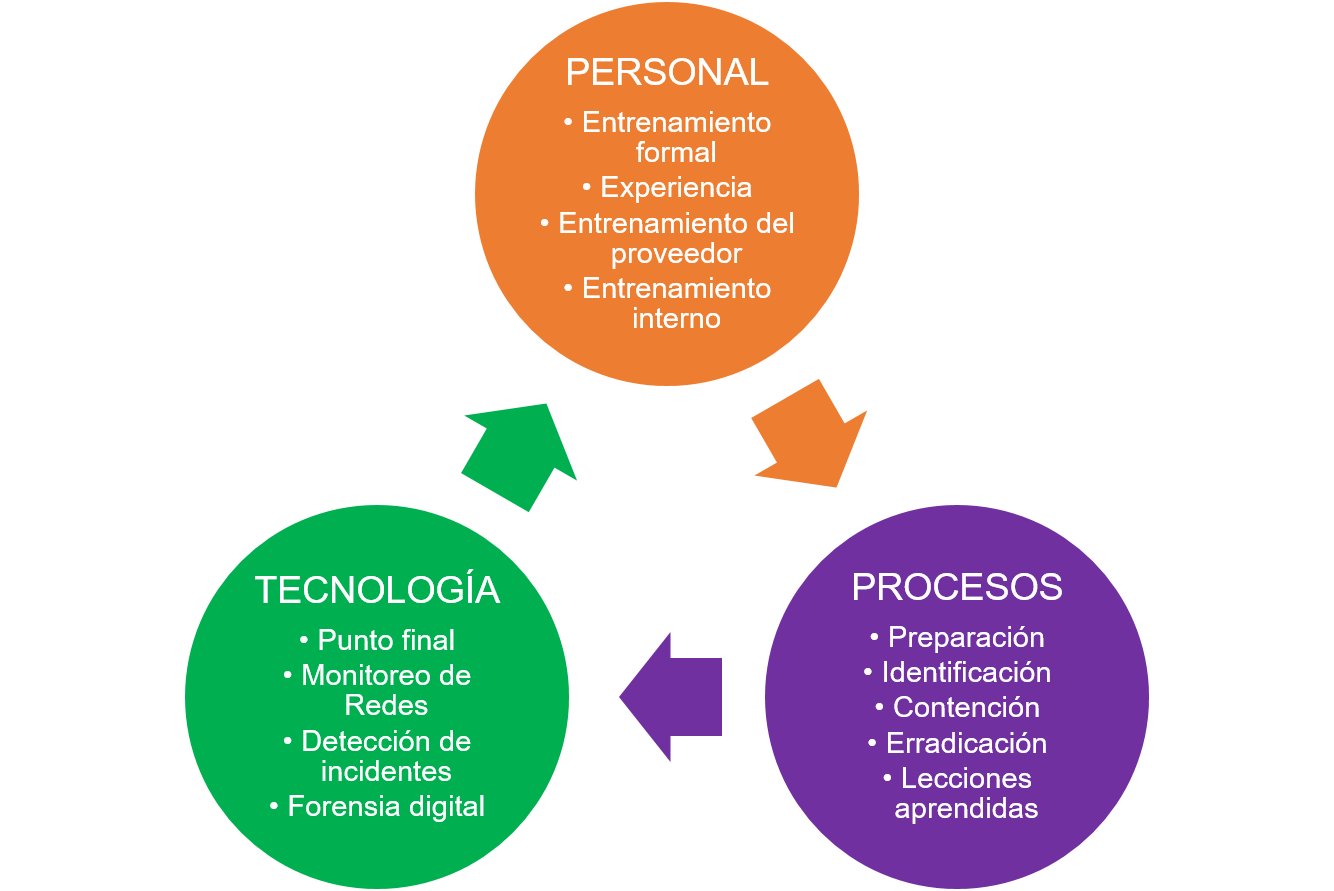
\includegraphics[width=1\textwidth]{./marco_teorico_imagenes/figura_1_pilares.png}
            \caption{Pilares de un CSIRT}
            \label{fig:pilares}
        \end{figure}
        Las infracciones a las políticas de seguridad y los ataques han concentrado la atención sobre las capacidades de detección, investigación y mitigación de incidentes de seguridad de la información en  las organizaciones. Si bien no siempre es posible evitar un incidente de seguridad, es necesario detectar y responder rápidamente para minimizar el daño. Para ello, es preciso realizar inversiones inteligentes basadas en un plan de seguridad que comprenda la realidad y necesidades específicas de la organización, ya que un gran monto de dinero o equipos adquiridos por si mismos no garantizan una mayor protección. \par
        Este plan debe incluir personal especializado, procedimientos e infraestructura  adaptados a la organización, con una gestión de objetivos a cumplir a corto, mediano y largo plazo. \par
        Para las organizaciones que no cuentan con una capacidad de manejo de incidentes, la creación desde cero de un Computer Security Incident Response Team (CSIRT) puede ser un proceso complejo y costoso. Sin embargo, no es necesario una gran inversión para obtener las capacidades elementales ofrecidas por un CSIRT, ya que es posible desarrollar una solución específica y a escala de la organización. \par
        Una vez identificadas las necesidades de la organización, el proceso de creación del CSIRT requiere de la creación, colaboración y comunicación entre los tres pilares que lo componen: el personal, la tecnología y los procesos, como se muestra en la Figura \ref{fig:pilares}. \par
        
        
        %\par
        El CSIRT debe tener una perspectiva flexible y escalable para mantener el ritmo de las tácticas de los adversarios, acompañando el crecimiento y evolución de la organización. \par
    \end{section}
    
   \begin{section}{Personal}  
   En cuanto al personal, estos comprenden tanto a los encargados de dar respuesta a los incidentes como a los analistas del CSIRT. Si bien la propia organización puede designar a sus integrantes para asumir estas funciones, existen otras alternativas como la tercerización mediante empresas especializadas que proveen el servicio de Managed Security Service Provider (MSSP) o contratar especialistas en respuesta a incidentes en el caso de una emergencia o un problema complejo. Otra vía consiste en la creación de equipos híbridos compuestos por personal perteneciente a la organización y especialistas externos. \par
    De acuerdo a una encuesta del SANS Institute del año 2014 \cite{sans_1}, el 61\% de las organizaciones relevadas manifestaron haber recurrido a personal de emergencia para cubrir incidentes críticos y el 58 \% tenía un equipo de respuesta propio. Por lo que las organizaciones no siempre cubren sus necesidades con miembros de su propio personal y en algunos casos las tareas recaen por completo en los servicios de terceros. Esto se debe a que, sin importar la estructura del equipo, el personal de un CSIRT debe contar con el entrenamiento necesario para tratar con los cambios en las amenazas a las que se enfrenta. En el Cuadro \ref{table:1} se muestran las responsabilidades y la formación requerida para cada uno de los integrantes de un CSIRT. \par
    
    \begin{table}%[ht]
    \centering
        \begin{tabular}{ | m{10em} | m{16em}| m{11em} | } 
            \hline
            Título profesional & Tarea & Entrenamiento requerido \\ 
            \hline
            Nivel 1 - Analista de alertas & Supervisa continuamente la cola de alertas, monitorea el estado de los sensores y los puntos finales, clasifica las alertas de seguridad y recopila los datos necesarios para iniciar el trabajo de Nivel 2. & Procedimientos de triage de alerta y detección de intrusos. Gestión de redes, información de seguridad y eventos. Capacitación en investigación basada en host. \\ 
            \hline
            Nivel 2 - Analista de respuesta a incidentes & Realiza un análisis profundo de incidentes al correlacionar datos de varias fuentes y determina si un sistema crítico o un conjunto de datos se ha visto afectado. Asesora sobre su remediación. & Análisis avanzado de forensia de redes y basado en host. Procedimientos de respuesta a incidentes, revisiones de registros, evaluación básica de malware e inteligencia de amenazas. \\ 
            \hline
            Nivel 3 - Especialista en la materia & Se trata de un conjunto de especialistas que cubren distintas áreas de un CSIRT. 
            Actúan como “cazadores” de amenazas, sin esperar que se intensifiquen los incidentes. Se encuentra estrechamente involucrado en el desarrollo, ajuste e implementación de análisis de detección de amenazas.
             & Entrenamiento avanzado en detección de anomalías. Entrenamiento específico en herramientas para la agregación y análisis de datos e inteligencia de amenazas. 
            Poseen un conocimiento profundo en áreas como redes, puntos finales, inteligencia de amenazas, forensia e ingeniería inversa de malware, así como la infraestructura de IT subyacente.
            \\ 
             \hline
            Director del CSIRT & Administra recursos para incluir personal, presupuesto, programación de turnos y estrategias para cumplir con los acuerdos de nivel de servicio. Se comunica con la gerencia y sirve como persona de contacto en el caso de incidentes críticos. Proporciona una dirección general para el CSIRT. & Gestión de proyectos, formación en gestión de respuesta a incidentes, habilidades generales de gestión de personas y comunicación institucional.  \\
            \hline %linea final de tabla
        \end{tabular}
        \caption{Integrantes de un CSIRT y sus funciones}
        \label{table:1}
    \end{table}
    \FloatBarrier % obliga a la imagen a renderizarse antes de este punto
        Para organizar el trabajo de los analistas, un CSIRT necesita un director que coordine los múltiples esfuerzos dentro y fuera del equipo. Su responsabilidad es dirigir el trabajo y organizar los recursos con el fin de detectar, investigar y priorizar incidentes que puedan impactar en la organización. Otra de las misiones asignadas al director consiste en desarrollar un modelo de flujo de trabajo e implementar procedimientos operativos estandarizados, para el proceso de manipulación de incidentes, que guíen a los analistas en la clasificación y respuesta apropiada.
        En la Figura \ref{fig:org_csirt} se observa un modelo de organización de un CSIRT.
        
        \begin{figure}[H]
            \centering
            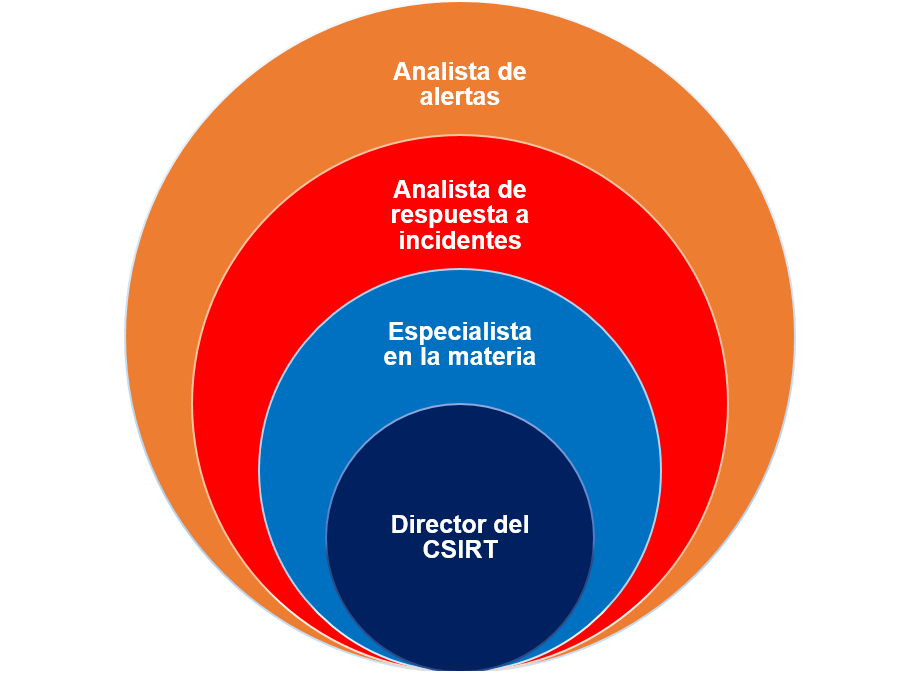
\includegraphics[width=1\textwidth]{./marco_teorico_imagenes/figura_2_org_csirt.png}
            \caption{Organización de un CSIRT}
            \label{fig:org_csirt}
        \end{figure}

   \end{section}
   
   \begin{section}{Procesos}  
        Para estandarizar las acciones que pueden tomar los analistas del CSIRT y asegurar que no se perderán tareas importantes en el camino, es necesario definir procesos repetibles de clasificación de incidentes e investigación. Al crear un flujo repetible de gestión de incidentes, se definen las responsabilidades y acciones de los miembros del equipo: desde la creación de una alerta y evaluación por analistas de nivel 1, hasta el tratamiento del incidente por parte del personal de los niveles superiores. Como consecuencia, la segmentación del proceso permite una gestión eficiente de los recursos del CSIRT. \par
    	Uno de los modelos de procesos de respuesta a incidentes más utilizado es el modelo DOE/CIAC \cite{doe_ciac}, que consiste en seis etapas: preparación, identificación, contención, erradicación, recuperación y lecciones aprendidas.

   \end{section}
   \begin{section}{Tecnología}
        En el núcleo de un CSIRT se encuentran las tecnologías de recolección de datos, agregación, detección, análisis y administración. En cuanto a la recolección, se trata de un sistema de monitoreo que obtiene sus datos a partir de un conjunto variado de fuentes como puntos finales (PC, dispositivos móviles, servidores, etc), redes, generadores de logs y eventos. Como resultado de la disponibilidad de los datos, antes y durante el incidente, los analistas pueden utilizar el sistema de vigilancia como una herramienta de investigación, revisando las actividades sospechosas del incidente en curso. Por otro lado, el sistema de monitoreo puede ser utilizado para generar la respuesta al incidente y potencialmente mitigar sus causas. \par
        Un aspecto importante a considerar es la compatibilidad de las tecnologías empleadas, en particular si la organización ya cuenta con una herramienta de monitoreo existente y se busca incorporar nuevas soluciones para integrarlas a los sistemas en servicio. En la Figura \ref{fig:comp_tech} se ejemplifica la necesidad de compatibilidad entre sistemas y componentes. 
        
        \begin{figure}[H]
            \centering
            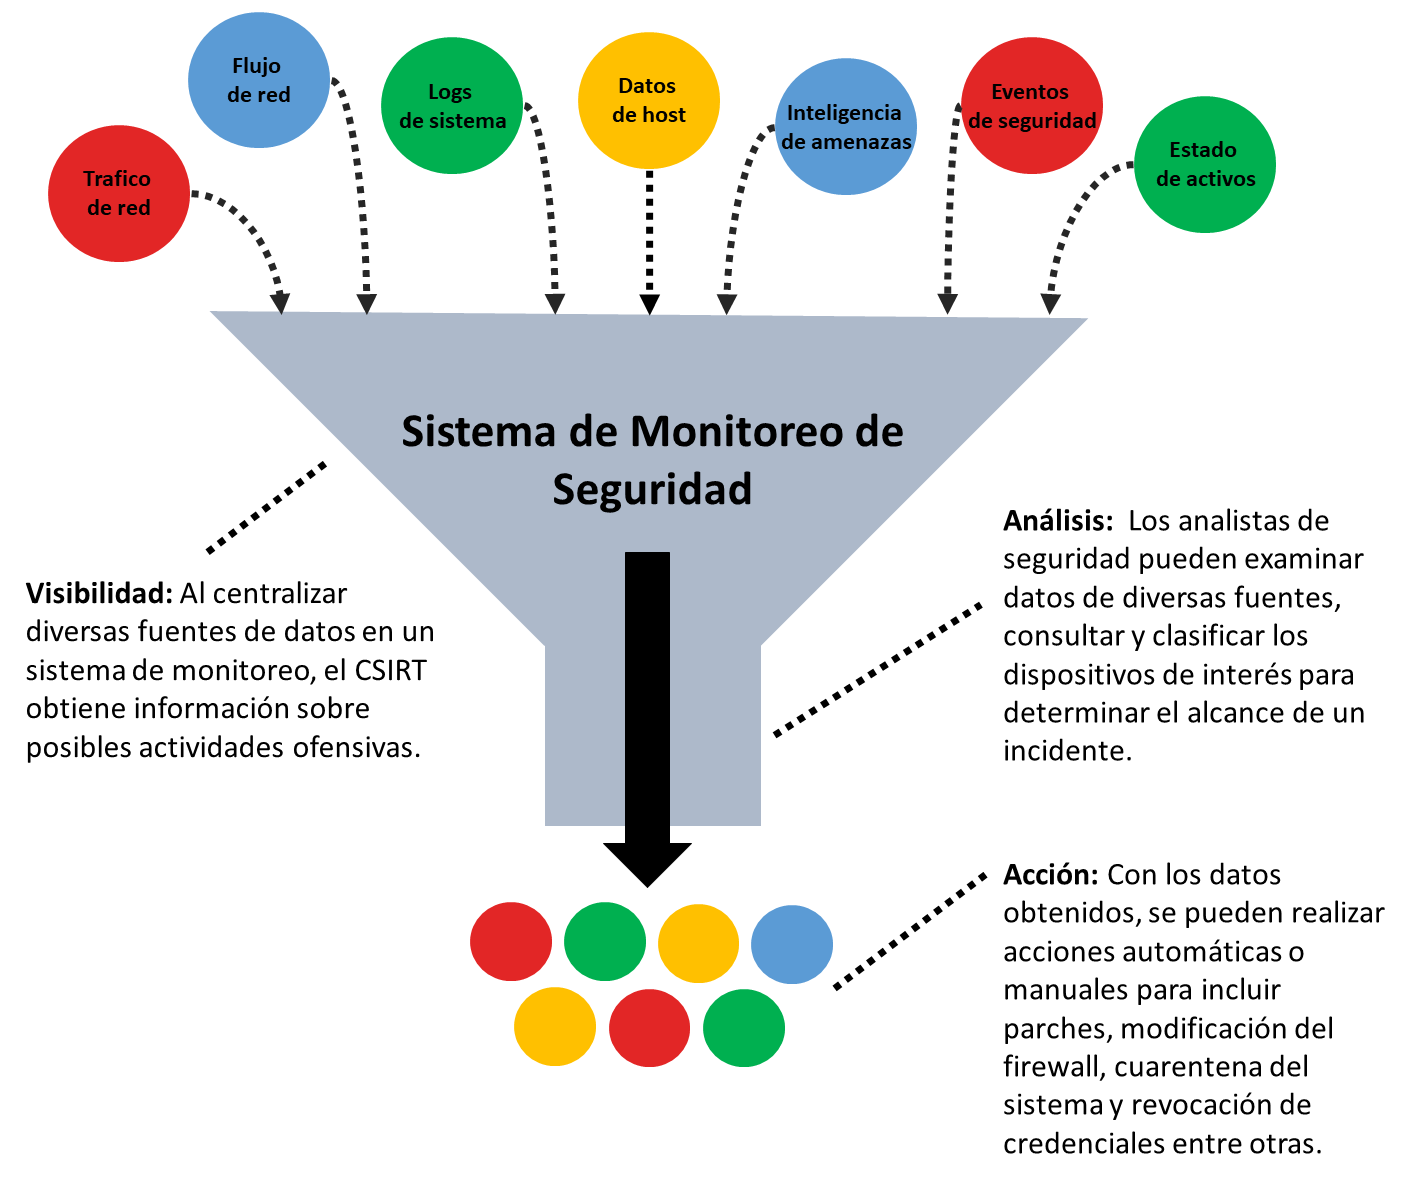
\includegraphics[width=1\textwidth]{./marco_teorico_imagenes/figura_3_compatibilidad_entre_tecnologias.png}
            \caption{Compatibilidad entre tecnologías de detección}
            \label{fig:comp_tech}
        \end{figure}
        \FloatBarrier
        \begin{subsection}{Agregando contexto a los incidentes}
        La incorporación de inteligencia de amenazas y otras informaciones de contexto tales como activos e identidades, contribuye al proceso de investigación del analista de un CSIRT. En determinados casos, la información inicial que está asociada a una alerta puede ser muy limitada, por ejemplo la dirección IP del punto final sospechoso es insuficiente por sí sola para tomar una decisión. \par
        Para que los analistas puedan investigar un incidente, generalmente necesitan más información, por ejemplo los nombres del dueño y de dominio de la máquina, registros DHCP para mapear la IP con el host al momento del incidente, etc. Si el sistema de monitoreo incorpora información de identidad y de los activos de información, entre otros datos de contexto, le permitirá al analista ahorrar tiempo y esfuerzo para priorizar los incidentes y elaborar la respuesta más apropiada.\par

        \end{subsection}
        \begin{subsection}{Definición de conductas normales}
        Dado que es posible observar patrones de comportamiento en usuarios, aplicaciones, infraestructura, redes y dispositivos, es útil establecer una referencia o línea base de la actividad de lo que se considerará un comportamiento normal. Esto facilitará la detección de conductas sospechosas anticipando posibles amenazas. \par
        Un sistema de monitoreo configurado y con una base de referencia adecuada estará en condiciones de enviar alertas confiables al analista de primer nivel. Esto obtiene especial relevancia, ya que de acuerdo al citado informe del SANS Institute del año 2014 \cite{sans_1}, uno de los principales desafíos en la utilización de registros de eventos de seguridad, es la incapacidad de distinguir actividades sospechosas de las normales. La ausencia de una referencia de “normalidad” es un obstáculo común al que se enfrentan las empresas de monitoreo y muchas organizaciones. \par
        La mejor práctica es utilizar plataformas que pueden crear líneas o patrones de referencia mediante el monitoreo de la red y la actividad de los puntos finales durante un periodo de tiempo.
        \end{subsection}
        
        \begin{subsection}{Inteligencia de amenazas}
        Los CSIRT bien establecidos o maduros desarrollan continuamente la capacidad de aprovechar la inteligencia de información proveniente tanto de sus incidentes pasados como de fuentes de inteligencia compartidas. Ejemplos de estas últimas son los proveedores especializados, CSIRT aliados, divisiones policiales de cibercrimen, organizaciones de intercambio de información como la Information Technology - Information Sharing and Analysis Center (IT-ISAC) \cite{it_isac}, etc. \par
        La capacidad de utilizar la inteligencia de amenazas contribuye a mejorar la precisión de la detección. De esta manera, es posible detectar patrones de amenazas ocultas en puntos finales, logs y registros de red, reduciendo las oportunidades de desarrollo de un ataque.
        \end{subsection}
      
        \begin{subsection}{Obstáculos para el manejo eficiente de incidentes del CSIRT}
        Algunos de los obstáculos que deben ser evitados por un CSIRT son aquellos que generan cuellos de botella en el proceso de respuesta a incidentes.  Este proceso que consiste en el traslado de un incidente entre los sucesivos niveles del CSIRT, eventualmente puede generar “ruido blanco”: la presencia de una gran cantidad de alertas de poca importancia y / o falsos positivos. De prolongarse esta situación en el tiempo, se produce un fenómeno llamado “fatiga de alertas” que afecta a los analistas provocando una disminución en sus capacidades de atender incidentes prioritarios. \par
        Al momento de elegir una herramienta de monitoreo, se debe considerar que incluya entre sus características la personalización del umbral de alertas y la posibilidad de combinar distintas alertas en un mismo incidente. Una herramienta de este tipo permite a los analistas clasificar las alertas más rápido, reduciendo las capas de evaluación necesarias antes de que el evento pueda ser confirmado y mitigado. 
        \end{subsection}
   \end{section}
      
   \begin{section}{Ámbitos de actuación de los CSIRT}
        En la actualidad existen en todo el mundo CSIRT pertenecientes a organizaciones que responden a distintos ámbitos de la sociedad y de diferente naturaleza (pública o privada). En términos generales, estos equipos se clasifican dependiendo de la comunidad a la que atienden, diferenciándose entre:
        \begin{itemize}
            \item \textbf{CSIRT para el sector de PYMES:} En este caso, el tamaño de las empresas hace poco viable que las organizaciones de este sector puedan implementar de forma individual las funciones de un CSIRT. Por lo tanto, surge la necesidad de unificar esfuerzos y servicios en un solo equipo capaz de dar soporte a varias empresas. La naturaleza de estos CSIRT puede ser pública o privada, dependiendo del contexto en el que se encuentren estas compañías.
            \item \textbf{CSIRT académico:} El área de responsabilidad de este tipo de equipos se circunscribe a instituciones académicas. Su tamaño, por lo tanto, puede variar dependiendo de las dimensiones de la comunidad, condicionando los servicios que ofrezcan, el modo en que lo hagan y su grado de intervención.
            \item \textbf{CSIRT comercial:} estos centros prestan distintos servicios a cambio de una contraprestación económica. Se trata de empresas especializadas en la industria de la ciberseguridad, que habitualmente utilizan acuerdos de servicios específicos con cada cliente.
            \item \textbf{CSIRT de proveedor:} se centra en los productos o servicios específicos de un proveedor. Su objetivo es proveer servicios y soluciones para eliminar o reducir el impacto negativo de las vulnerabilidades en estos últimos, ya sea un producto tecnológico o un servicio TIC.
            \item \textbf{CSIRT del sector militar:} Prestan servicios a organizaciones militares, con responsabilidades en infraestructuras TIC necesarias para la Defensa. Su comunidad está conformada por las instituciones militares y de entidades estrechamente relacionadas con éstas. Por ejemplo, en nuestro país el Comando Conjunto de Ciberdefensa \cite{fa_comando}, es el encargado de la defensa de la infraestructura de redes y activos de la información de las Fuerzas Armadas.
            \item \textbf{CSIRT para protección de infraestructuras críticas:}  Los CSIRT de este sector se centran principalmente en la protección de las infraestructuras críticas  y de los activos de información asociados. Ejemplos de infraestructuras críticas son las centrales y redes de energía, telecomunicaciones, sistema financiero, sector sanitario, agua, transportes, industria nuclear, etc.
            \item \textbf{CSIRT gubernamental:} Bajo esta denominación se sitúan los equipos cuyo principal objetivo es asegurar la infraestructura TIC de un Gobierno/Estado y los servicios ofrecidos a la población. La Comunidad a la que están dirigidos son las administraciones públicas y sus distintos organismos. Estos CSIRT gubernamentales generalmente forman parte de las instituciones del Estado.
            \item \textbf{CSIRT Nacional:} Este es un equipo con responsabilidad general de coordinación sobre todos los sectores y tiene una amplia responsabilidad sobre prácticamente todos los CSIRT tratados anteriormente. Este centro funciona como punto focal de contacto tanto en el entorno nacional como para requerimientos internacionales. ENISA, la Agencia de Ciberseguridad para la Unión Europea, define en un documento \cite{enisa} elaborado en diciembre de 2009, a este tipo de CSIRT como “aquel que actúa como el Point of Contact (POC) con otros equipos nacionales y/o internacionales. De hecho, podría considerarse como CSIRT  del último recurso, por su papel de coordinación”. Cada nación define la misión de estas unidades y establece sus operaciones, su organización y su imperativo legal en base a las necesidades del país y su comunidad. En Argentina, esta responsabilidad es asumida por la Dirección Nacional de Ciberseguridad \cite{dir_nac_ciber}. 
            \begin{figure}[H]
                \centering
              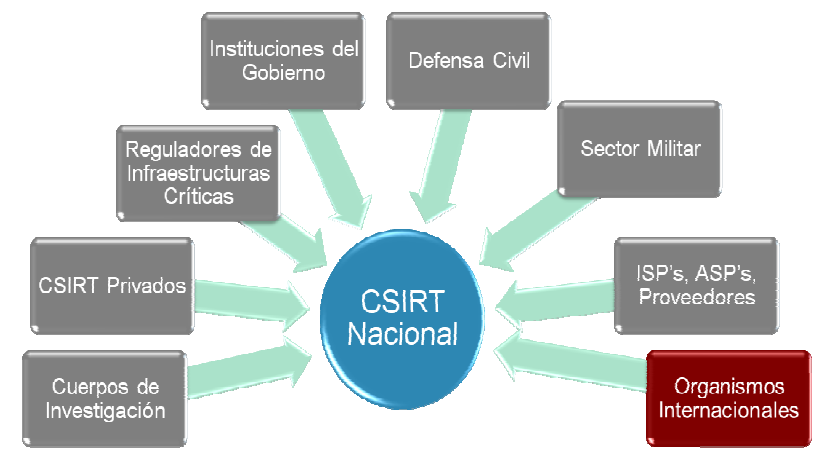
\includegraphics[width=0.8\textwidth]{./marco_teorico_imagenes/figura_4_csirt_nacional.png}
                \caption{CSIRT Nacional como centro de coordinación}
                \label{fig:csirt_nac}
            \end{figure}
            \FloatBarrier
            Frente a esto, todos los CSIRT nacionales tienen un objetivo común, mantener seguras las redes de sus países. De este modo podemos concluir que, aunque cada uno utiliza herramientas y procedimientos diferentes, todos comparten el mismo objetivo:
            \begin{enumerate}
                \item Designar un punto de contacto para la coordinación de la respuesta a incidentes.
                \item Construir y mantener una red de contactos extensa, tanto nacional como internacional.
                \item Monitorización de la situación actual y mejora de la concientización.
            \end{enumerate}
            Es importante destacar que la constitución de un CSIRT nacional o gubernamental, no es la única medida a tener en cuenta en una estrategia de ciberseguridad completa por parte de un Estado. Es una parte importante de la misma teniendo en cuenta, además, que este tipo de equipos deberían asumir la responsabilidad de la Protección de las Infraestructuras Críticas de Información (CIIP) del país.
        \end{itemize}
        \begin{subsection}{Estado de la ciberseguridad en Argentina} 
        Los orígenes de la gestión de la seguridad informática en nuestro país pueden rastrearse en el decreto 856/98 \cite{jef_gab_856_98} y a la Resolución de la Secretaría de la Función Pública (SFP), organismo dependiente de la Jefatura de Gabinete de Ministros, Res SFP 81/99 \cite{sub_tec}. Esta Resolución establece la reorganización de la Subsecretaría de Tecnologías Informáticas y el “Reglamento de Operación del ArCERT", donde se indican los requisitos y condiciones de operación de la Coordinación de Emergencia en Redes Teleinformáticas - ArCERT, y las Políticas de Seguridad del mismo. \par
        El objetivo principal del ArCERT fue coordinar y colaborar en los esfuerzos orientados a elevar los umbrales de seguridad en los recursos y en los sistemas de información en el ámbito de la Administración Pública Nacional (APN). Para esto se estableció una estrategia de coordinación, asesoramiento y capacitación hacia los organismos públicos en la gestión de la problemática de seguridad. \par
        Sus funciones \cite{sub_tec} eran: 
        \begin{enumerate}
            \item Proveer un servicio especializado de asesoramiento en seguridad de redes.
            \item Promover la coordinación entre los organismos de la Administración Pública Nacional para prevenir, detectar, manejar y recuperar incidentes de seguridad.
            \item Centralizar los reportes sobre incidentes de seguridad ocurridos en la APN y facilitar el intercambio de información para afrontarlos.
            \item Actuar como repositorio de toda la información sobre incidentes de seguridad, herramientas, técnicas de protección y defensa.
        \end{enumerate}
        En el marco de las funciones nombradas, el ArCERT realizó actividades de investigación de amenazas y nuevas soluciones disponibles,  divulgación de incidentes y soluciones así como capacitaciones de seguridad en redes y seminarios de actualización periódicos. \par
        El año 2011 marcó el comienzo de un largo proceso de reestructuración de los organismos del Estado Nacional relativos a la ciberseguridad, que incluyó el reordenamiento de estructuras internas, la creación de nuevas dependencias y el reemplazo o absorción de unidades preexistentes por las de nueva formación. Ese mismo año, mediante la resolución de la Jefatura del Gabinete de Ministros, Res JGM Nº 580/2011 \cite{jef_gab_crease} se creó el Programa de Infraestructuras Criticas de Informacion y Ciberseguridad, que declaró como finalidad “Impulsar la creación y adopción de un marco regulatorio específico que propicie la identificación y protección de las Infraestructuras estratégicas y críticas del Sector Público Nacional, los organismos interjurisdiccionales y las organizaciones civiles y del sector privado que así lo requieran”. \par
        En el año 2013 y mediante el artículo 1º de la Disposición Nº 2/2013 \cite{disp_2_2013} de la Oficina Nacional de Tecnologías de Información (ONTI), se creó el Instituto de Ciencias e Ingeniería de Computación - Computer Emergency Response Team (ICIC-CERT) que reemplazó al ArCERT. \par
        Este nuevo CERT heredaba parte de las responsabilidades del original, a la par que otros artículos de la referida disposición creaban nuevos grupos de trabajo especializados que ampliaban las capacidades, funciones y responsabilidades concentradas originalmente en el ArCERT, tales como el grupo ICIC - GAP (Grupo de Acción Preventiva, art. 3º) con funciones similares a las encargadas al ArCERT pero enfocadas a monitorear “los servicios que el Sector Público Nacional brinda a través de la red de Internet y aquellos que se identifiquen como Infraestructura Crítica para la prevención de posibles fallas de Seguridad”, el grupo “ICIC - GICI” (Grupo de Infraestructuras Críticas de Información, art. 4º) especializado en el desarrollo y aplicación de nuevas tecnologías para el monitoreo, simulación y respuesta a incidentes en la red de infraestructuras críticas, establecer prioridades y planes estratégicos para liderar el abordaje de la ciberseguridad para la protección de este tipo de infraestructuras, coordinar la implementación de ejercicios de respuesta ante la eventualidad de un intento de vulneración de estos activos, entre otras. Finalmente, se creó el grupo de trabajo “ICIC - INTERNET SANO” (art. 7º) con el objetivo específico de ocuparse de las tareas de difusión y capacitación que anteriormente le correspondía al ArCERT. En cuanto al programa de infraestructuras críticas, podemos mencionar la adhesión de la Universidad Nacional de Córdoba, cuando el 15 de Julio de 2014, mediante la Resolución 1221 \cite{unc_rec} firmada por el Rector Tamarit, en su artículo N°1 “Hacer lugar a lo solicitado a fS.1 por la Prosecretaría de Informática y, en consecuencia, adherir al "Programa Nacional de Infraestructuras Críticas de Información y Ciberseguridad"...” \par
        El Estado Nacional siguió actualizando sus políticas en los años siguientes, creando nuevos centros de respuesta a incidentes y actualizando la normativa vigente. Algunos de los ejemplos son la creación del Comando Conjunto de Ciberdefensa de las Fuerzas Armadas \cite{fa_comando}, el “MING-CSIRT” \cite{minis_seg} del Ministerio de Seguridad de la Nación, la Dirección Nacional de Ciberseguridad \cite{dir_nac_ciber} y sus correspondientes unidades de gobierno. \par
       \begin{figure}[H]
            \centering
            \subfloat[\centering] {{
\includegraphics[width=5 cm, valign=c]{./marco_teorico_imagenes/figura_5a_comando_conjunto.png}}} %
            \quad
            \subfloat[\centering] {{
\includegraphics[width=5 cm, valign=c]{./marco_teorico_imagenes/figura_5b_csirt_neuquen.png}}} %
            \caption{Insignias de CSIRTS argentinos: (a) corresponde al Comando Conjunto de Ciberdefensa y (b) corresponde al CSIRT de la provincia de Neuquén}
            \label{fig:ciberdef_nqn}
        \end{figure}
        \FloatBarrier
        Por otro lado, los Estados Provinciales, universidades y empresas también han desarrollado e implantado CSIRTs en sus organizaciones. Algunos ejemplos de esto son el “BA-CSIRT”\cite{ba_csirt} de la Ciudad de Buenos Aires, el “CSIRT-NQN”\cite{nqn_csirt} del gobierno de la provincia de Neuquén, “CERT UNLP” \cite{unlp_cert} de la Universidad Nacional de La Plata o el que dispone NIC Argentina \cite{nic_arg} destinado a la infraestructura crítica de DNS. En el caso de las empresas, podemos mencionar a los CSIRT de las redes bancarias Link \cite{red_link} y Banelco\cite{banelco}.
            \begin{subsubsection}{Demanda de ciberseguridad Argentina}
            Nuestro país, de manera análoga a los demás países de la región, ha experimentado un crecimiento exponencial de incidentes de ciberseguridad a lo largo de las últimas dos décadas. Esto afecta a individuos, empresas, universidades, infraestructuras críticas y a los organismos de diferentes niveles del gobierno. Este incremento exponencial en la demanda de ciberseguridad no ha encontrado una respuesta adecuada del Estado Argentino. Un ejemplo lo constituyen los 1590 millones de ataques[19] que sufrió el sistema bancario argentino en el año 2019 o los 187 millones de ciberataques entre enero y marzo del 2020 con un incremento del 131\% solo para el mes de marzo, según la plataforma “Fortinet Threat Intelligence Insider Latin America”[20]. \par 
            En la Figura 6 se observan las diez amenazas más frecuentes y la cantidad de ataques producidos en Argentina por ellas, en el periodo comprendido entre los meses de abril y junio de 2020. Los tres primeros corresponden al troyano de puertas traseras “DoublePulsar Backdoor”, negociación de cifrados SSL anónimos e intentos de ataque contra una vulnerabilidad de divulgación de información en el servidor SMB de Microsoft Windows. La fuente es un informe de Fortinet Threat Intelligence Insider Latin America [20].\par

            \end{subsubsection}
        \end{subsection}
   \end{section}

    \begin{section}{SIEM: Definición y funciones}
    
    \end{section}
    \begin{section}{Soluciones disponibles}
    
    
        \begin{subsection}{Soluciones comerciales}
        
        \end{subsection}
        \begin{subsection}{Soluciones gratuitas y de código abierto}
        
        
            \begin{subsubsection}{AlienVault OSSIM}
            
            \end{subsubsection}
            \begin{subsubsection}{Graylog}
            
            \end{subsubsection}
            \begin{subsubsection}{Elastic Stack}
            
            \end{subsubsection}
            \begin{subsubsection}{Security Onion}
            
            \end{subsubsection}
            
        \end{subsection} 
    \end{section}
    \begin{section}{Corolario}
    
    \end{section}
            
            
            
            
